\section{Hướng dẫn sử dụng ứng dụng}
\subsection{Cài đặt và khởi chạy server}
\begin{enumerate}
\item Cài đặt các thư viện cần thiết:
\lstset{style=mystyle}
\begin{lstlisting}[language=bash]
pip install -r requirements.txt
\end{lstlisting}

\item Cài đặt VnCoreNLP cho quá trình pre-processing trước khi đưa dữ liệu vào mô hình để dự đoán.

\lstset{style=mystyle}
\begin{lstlisting}[language=bash]
bash vncorenlp.sh
\end{lstlisting}

\item Download model đã được train tại  \href{https://drive.google.com/drive/u/2/folders/19AGLo-27EeuXDkKG2JstuCgrcwB0854r}{link này}

\item Sau khi download model, ta giải nén model vào thư mục \texttt{model-save} sao cho cây thư mục của project có dạng như sau:
\lstset{style=mystyle}
\begin{lstlisting}[language=bash]
DemoViHealthBERT-NER
|   .gitignore
|   main.py
|   data_loader.py
|   readme.md
|   requirements.txt
|   vncorenlp.sh
+---model
|       module.py
|       vihnbert.py
+---model-save
|       config.json
|       eval_dev_results.txt
|       eval_test_results.txt
|       events.out.tfevents.1667922466.cb80415698cc.105.1
|       pytorch_model.bin
|       training_args.bin
+---web-demo-ner
|
\---vncorenlp
    |   VnCoreNLP-1.1.1.jar
    |
    \---models
        \---wordsegmenter
                vi-vocab
                wordsegmenter.rdr
\end{lstlisting}

\item Khởi chạy server
\lstset{style=mystyle}
\begin{lstlisting}[language=bash]
python main.py 
\end{lstlisting}
\end{enumerate}
\subsection{Cài đặt phần ứng dụng Web.}
\begin{enumerate}
\item Cài đặt Flutter SDK tham khảo tại \href{https://docs.flutter.dev/get-started/install}{link}.
\item Cập nhật phiên bản mới nhất của Flutter SDK.
\lstset{style=mystyle}
\begin{lstlisting}[language=bash]
flutter channel stable
flutter upgrade
\end{lstlisting}
\item Liệt kê danh sách các device có thể sử dụng để chạy ứng dụng Flutter.
\begin{lstlisting}[language=bash]
flutter devices
\end{lstlisting}
 Ở đây nhóm sử dụng \texttt{chrome} trong danh sách connected devices, ngoài ra cũng có thể sử dụng \texttt{edge} hoặc các thiết bị mobile (nếu có).

\item Chạy ứng dụng Web.
\begin{lstlisting}[language=bash]
cd web-demo-ner
flutter run -d chrome
\end{lstlisting}
\end{enumerate}
Tham khảo chi tiết hơn về xây dựng ứng dụng Web với Flutter tại \href{https://docs.flutter.dev/get-started/web}{link}.

\subsection{Demo}
Video demo của ứng dụng trên YouTube.

\begin{figure}
\centering
\resizebox{\textwidth}{!}{
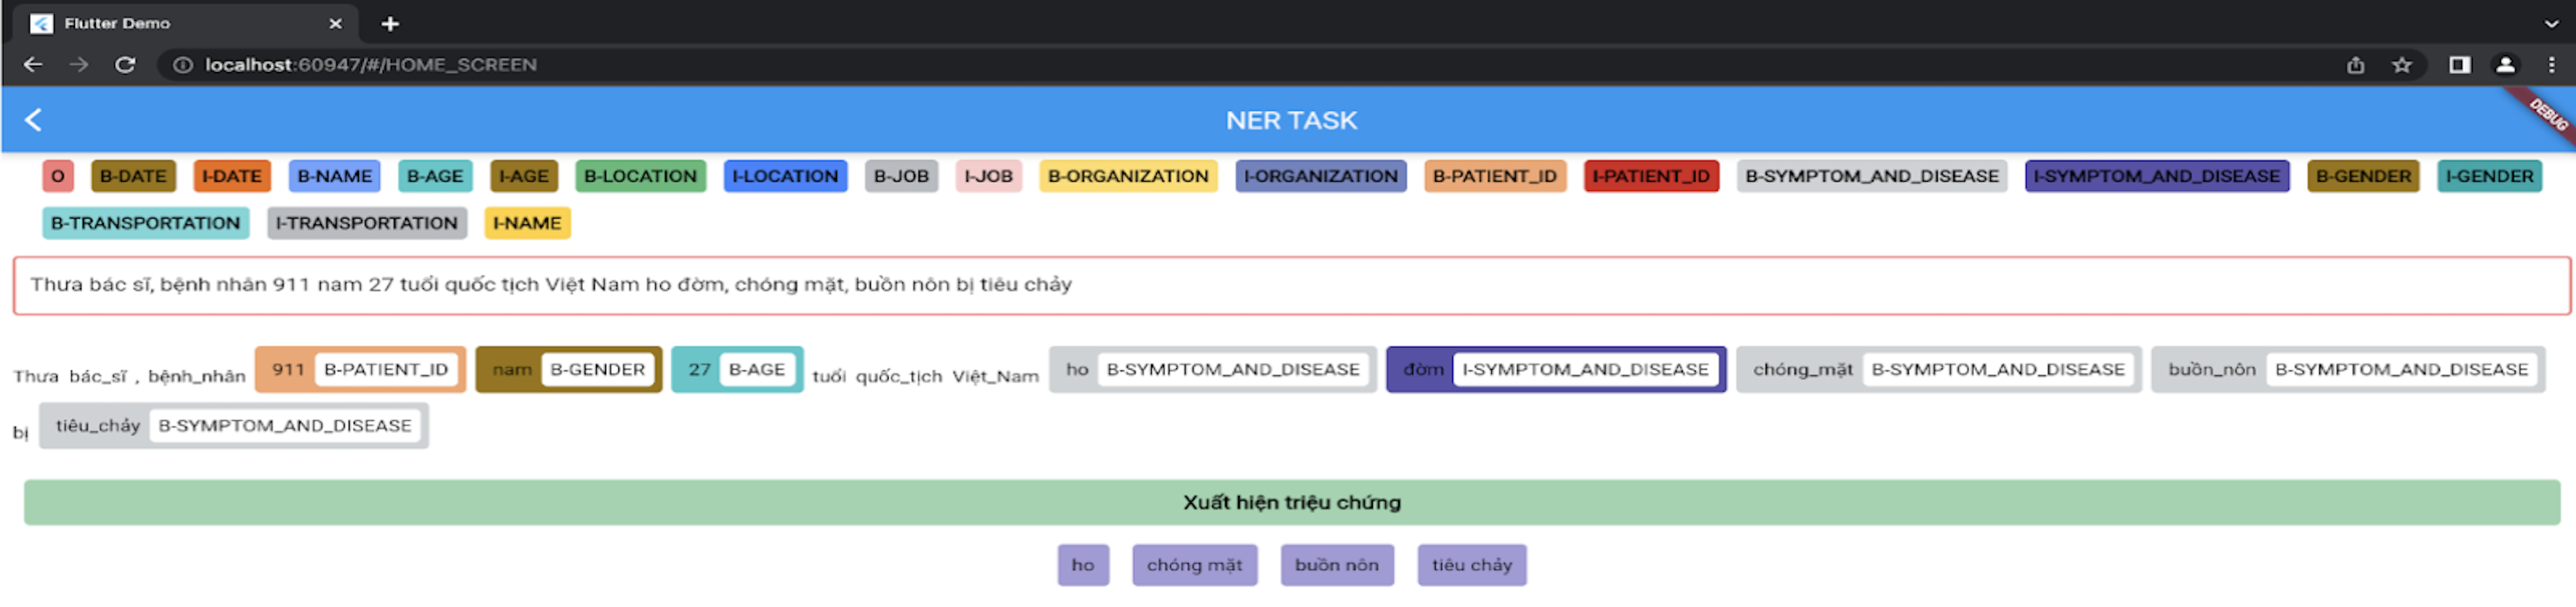
\includegraphics{img/Demo-web.png}
}
% 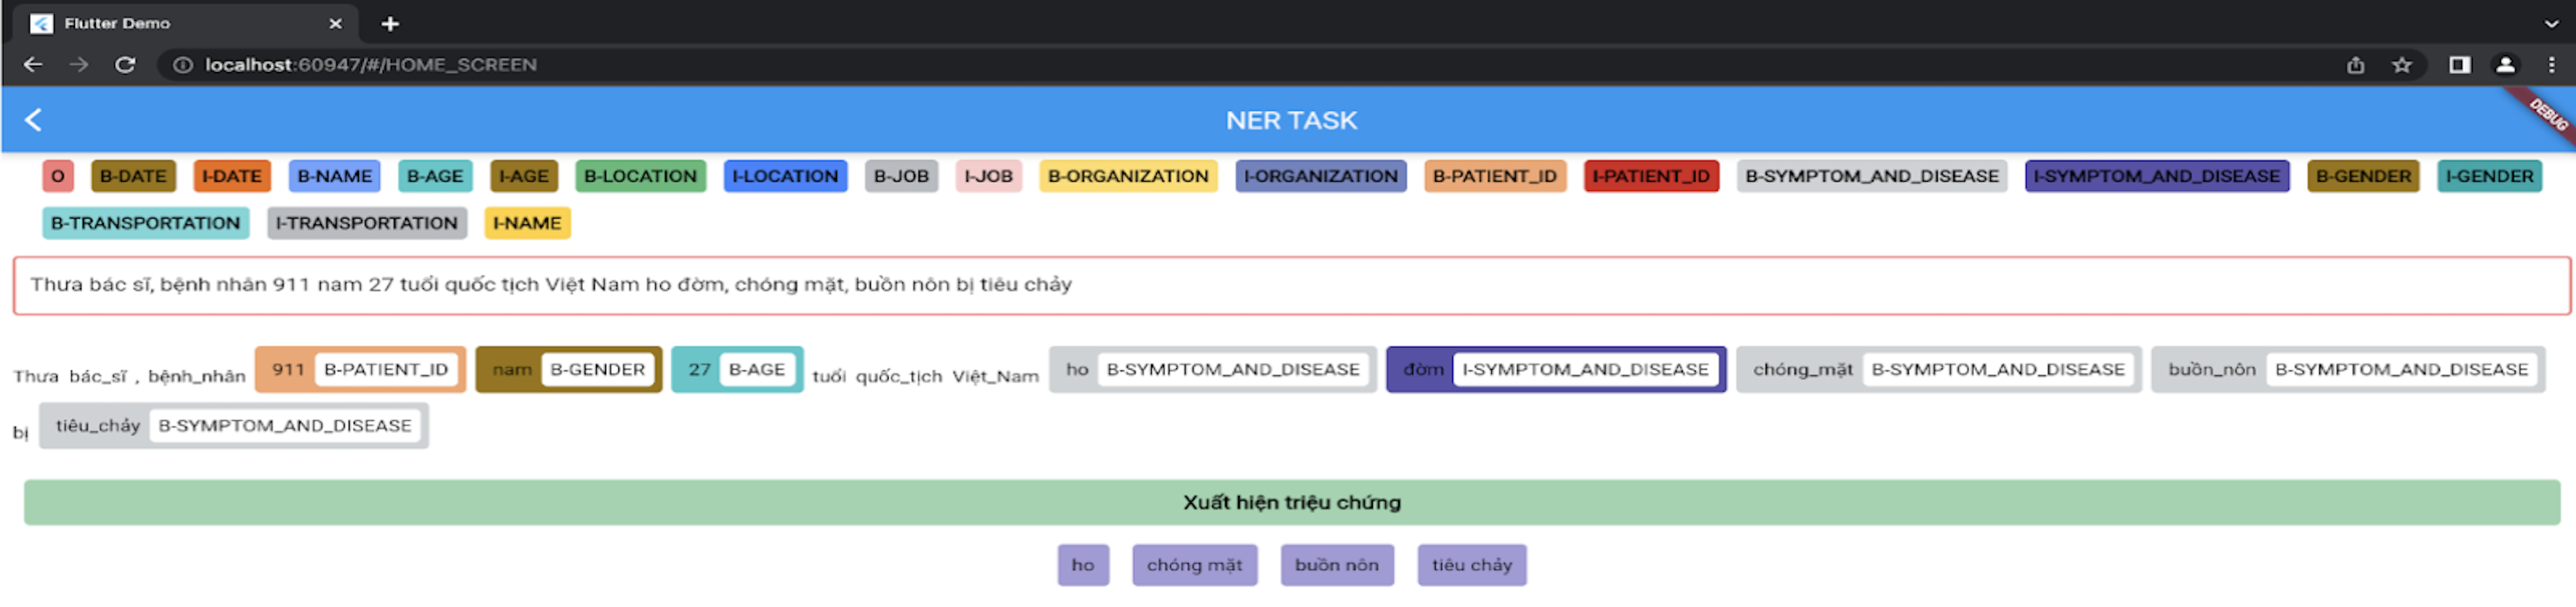
\includegraphics[scale=.25]{img/Demo-web.png}
\caption{Web trích xuất triệu chứng.}
\label{fig:web-demo}
\end{figure}